\section{Загальні відомості}

\vspace{-\baselineskip}

Структурне розпізнавання зображень зводиться до розв'язання специфічних
задач дискретної оптимізації \cite{SchlGig_1_usim2007, Boykov, Boykov_2, savchynskyy}. Незважаючи на велике різноманіття даних задач,
багато з них можна представити як \((\max,+)\) задачі розмітки.
До відшукання оптимальних розміток \((\max,+)\) задачі зводиться багато
прикладних задач структурного розпізнавання образів. Серед них сегментація,
стереозір, знешумлення, бінаризація та багато інших \cite{WANG20131610, Boykov_2, comp_vision}.

Далеко не завжди є можливість знайти точний розв'язок до
масштабних задач оптимізації. Всі прикладні задачі відносяться до цього класу.
За певних умов точний розв'язок можливий. Наприклад, алгоритм динамічного програмування
знаходить глобальний мінімум задачі за умови, якщо граф є ациклічною
структурою \cite{ten_lectures}. Для ациклічних моделей складність алгоритму росте пропорційно
розміру задачі.
На жаль, не для всіх прикладних задач можливий такий розв'язок.
Більш широким класом розв'язних задач є супермодулярні задачі. Супермодулярність
для \((\max,+)\) задач розмітки --- це свого роду ,,аналог'' опуклості функції в теорії
оптимізації. За таких умов існують алгоритми, які дозволяють знайти
точний розв'язок задачі за скінченну кількість кроків.
Відмітимо, що будь-яка задача на ациклічній структурі є супермодулярною.
% якщо впорядкованість міток відома, то можна min/max, ishikawa

\subsection{Частковий випадок на дві мітки}
Одним із перших алгоритмів розв'язування є алгоритм \cite{Greig_port}, який
дозволяє знаходити точний розв'язок \((\max,+)\) задачі розмітки при обмеженні, що
задача має лише 2 мітки. Прикладом такої задачі може бути задача знешумлення
бінарного зображення.
Ідея згаданого алгоритму полягає в тому, щоб
представити задачу як орієнтований граф спеціального виду таким чином, щоб
мінімальний зріз цього графу відповідав розв'язку прямої задачі розмітки.
В теорії графів існують алгоритми, які можуть знайти розв'язок за поліноміальний
час \cite{Boykov, Boykov_2, ford}. Суттєвим обмеженням алгоритму є те, що задача повинна містити лише 2 мітки.
На жаль, для більшості прикладних задач цього недостатньо.


\subsection{Зведення задачi до пошуку максимального потоку}

Підхід \cite{ishikawa} є у певному сенсі узагальненням попереднього алгоритму на довільну
скінченну кількість міток. Додатковою умовою застосування є відома впорядкованість
множини міток. Як і у попередньому методі, основна ідея  полягає в побудові
спеціального орієнтованого графу, який відповідає \((\max,+)\) задачі розмітки.
Розв'язком буде значення мінімального розрізу цього графу.

\begin{figure}[h]
  \centering
  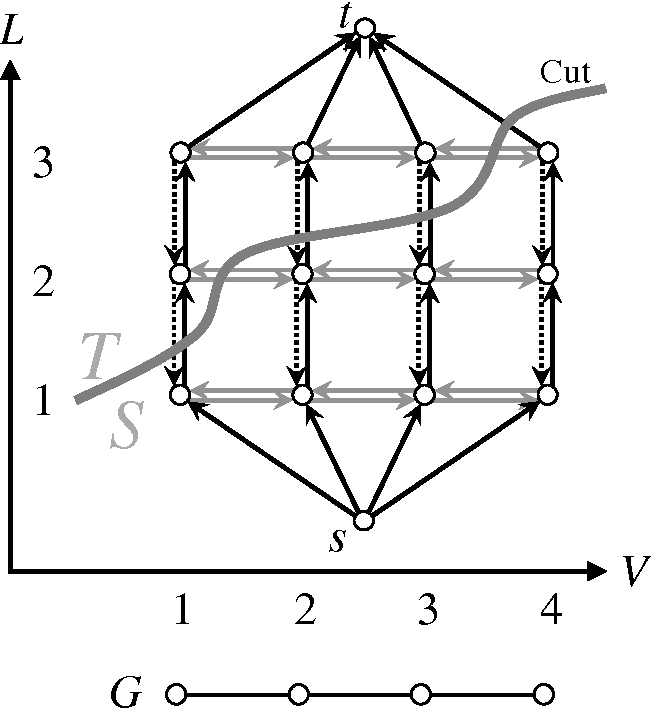
\includegraphics[width=0.4\textwidth]{images/ishikawa_graph.png}
  \caption{Приклад графу \cite{ishikawa}}
  \label{fig:graph_example}
\end{figure}


\subsection{Перетворення k в 2}

Перетворення k в 2 \cite{k22} дає можливість зводити супермодулярні задачі із
довільною кількістю міток до задач із двома мітками.
Суть підходу полягає в тому, що будь-яку \((\max,+)\) задачу розмітки можна
представити як бінарну задачу, а далі використати найменший розріз для знаходження
точного розв'язку. Отже, всі отримані результати для бінарних задач
узагальнюються до загального випадку \((\max,+)\) задачі розмітки із довільною
кількістю міток.

\subsection{Ітеративні методи}

Інший спосіб розв'язання \((\max,+)\) задач розмітки полягає у застосуванні
ітеративних алгоритмів. Часто ітеративні алгоритми застосовуються до цільової функції
двоїстої задачі оптимізації \cite{SchlGig_1_usim2007,diffusion_shlezinger}. Перевагою даного підходу є те, що ітеративні алгоритми
не накладають жорстких умов на вхідні дані задачі, тому
множина прикладних задач, до яких вони застосовні, розширюється.
Варто визнати, що не всі ітеративні
методи гарантовано дають точний розв'язок.
Деякі з них наближаються до точного розв'язку лише у ліміті,
що є недоліком з практичної точки зору.

Мінімізація цільової функції двоїстої задачі є доволі універсальним способом відшукання найкращої
нечіткої розмітки для довільної задачі \cite{diffusion_shlezinger,savchynskyy,SchlGig_1_usim2007}. Проте на даний момент існують лише окремі спроби вирішити цю задачу,
а практично гарні алгоритми невідомі.
Однією з таких спроб є алгоритм дифузії \cite{diffusion_shlezinger, savchynskyy}.
Відомо, що за скінченну кількість кроків алгоритм дифузії для будь-якої супермодулярної задачі
знайде рішення, яке відрізняється від найкращого не більше, ніж на $\varepsilon$,
для будь-якого наперед заданого $\varepsilon>0$.

\begin{figure}[h]
  \centering
  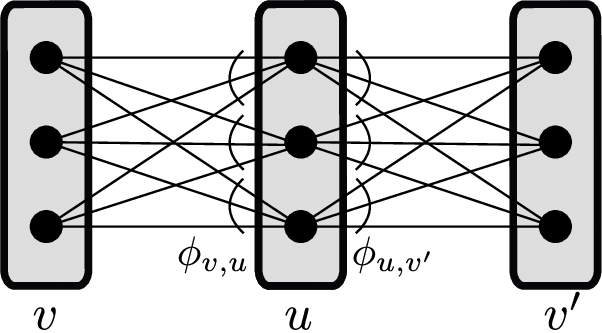
\includegraphics[width=0.4\textwidth]{images/One-elementary-step-of_diffusion.png}
  \caption{1 крок алгоритму дифузії --- оптимізація за блоком змінних \cite{ishikawa}}
  \label{fig:graph_example}
\end{figure}

Алгоритм дифузії дозволяє розв'язувати широкий клас задач, який містить всі
супермодулярні задачі. Проте немає гарантії знаходження мінімального
значення цільової функції двоїстої задачі. Цим недоліком володіють також
методи, що засновані на субградієнтній оптимізації \cite{Shor1985}.

Для субградієнтної оптимізації є додаткова складність у необхідності визначення
умови зупинки алгоритму та способі відшукання оптимальної розмітки
після досягнення оптимуму. Обидві ці проблеми частково вирішуються в \cite{lopatka_stop_cond}.

% \subsection{Висновки}

% У даному розділі описано методи, які по-різному підходять до
% розв'язування \((\max,+)\) задач розмітки. Звичайно, найбільш бажаними є методи,
% які знаходять точний розв'язок задачі, але, як бачимо, вони всі мають недоліки:
% додаткові обмеження, які накладаються на вхідні умови задачі, або розв'язок
% лише обмеженого класу задач, що на практиці часто звужує коло застосовності
% цих методів.

% На противагу прямим методам розв'язування ітеративні методи часто дозволяють
% знаходити розв'язок до більш широкого кола задач, не накладаючи додаткових
% обмежень. Недоліками цих методів часто є їх повільність та відсутність
% будь-яких гарантій на відшукання точного розв'язку, а також проблема відшукання
% оптимальної розмітки після досягнення прийнятного значення цільової функції.
% Для даних алгоритмів це є окремою задачею, яка часто є обчислювально більш
% складною, ніж сама оптимізація цільової функції.

% Нові методи розв'язування такого класу задач часто є спробами або розширити
% клас задач, які розв'язуються точно, або пришвидшити та вдосконалити
% ітеративні методи, надати їм теоретичні гарантії на відшукання
% прийнятного розв'язку.
